\documentclass[12pt,a4paper]{article}
\usepackage{cite}
\usepackage{fullpage}
\usepackage{indentfirst}
\usepackage{parskip}
\usepackage{amsmath}
\usepackage{hyperref}
\usepackage{bm}
\usepackage{enumerate}
\usepackage{enumitem}
\usepackage{graphicx}
\usepackage{booktabs}
\usepackage{url}
\usepackage[UTF8]{ctex}

\begin{document}
\setlength{\parindent}{2em}

\pdfbookmark[0]{Front page}{label:frontpage}%
\begin{titlepage}
  \noindent%
  \begin{tabular}{@{}p{\textwidth}@{}}
    \toprule[2pt]
    \midrule
    \vspace{0.2cm}\\
    \begin{center}
    \Huge{\textbf{
      基于AODV的支付通道网络\\路由协议 \\[8pt]
    }}
    \end{center}
    \begin{center}
      \Large{
        分布式计算课程主题报告
      }
    \end{center}
    \vspace{0.2cm}\\
    \midrule
    \toprule[2pt]
  \end{tabular}
  \vspace{5 cm}
  \begin{center}
    {\Large
      第15组
    }\\
    \vspace{0.2cm}
    {\Large
      1831605 \quad 刘诗洋 \\[5pt]
      1831606 \quad 陆思远 \\[5pt]
      1831607 \quad 余\quad豪 \\[5pt]
    }
  \end{center}
  \vfill
  \begin{center}
    {\Large
      同济大学\\[5pt]
      软件学院\\[5pt]
    }
  \end{center}
\end{titlepage}
\clearpage

\tableofcontents
\clearpage

\section{概述}
这篇报告是我们以论文 \cite{hoenisch2018aodv} 为基础,在较为充分的文献查阅及原理探究后,对支付通道网络及其路由协议做的内容梳理。我们从区块链的一大应用:加密货币开始,介绍其现状及共有问题。为了解决这些问题,研究者们提出了链下的支付网络,也即支付通道网络(Payment Channel Network, PCN),其中闪电网络(Lightning Network, LN)是较为突出的代表。但以主动式路由为路由协议的LN存在一些固有局限,为了发挥PCNs的潜力,研究者提出了以AODV(Ad-hoc On-demand Distance Vector)为基础的被动式路由协议,以期有效地解决问题。基于以上问题和解决方案,我们的报告内容也将按这一顺序展开,具体为:
\begin{itemize}
	\item 区块链及其应用的发展、愿景及问题;
	\item 闪电网络;
	\item 支付通道网络的特性、问题及需求;
	\item 路由协议及其种类简介;
	\item 基于AODV的路由协议及算法详述;
	\item 网络及协议性能评价;
	\item 总结与展望。
\end{itemize}

\section{区块链的发展、目标与问题}
随着比特币 \cite{nakamoto2008bitcoin} 以及其他诸多电子加密货币的出现,区块链一词逐渐被人们所知。作为比特币背后的技术基础,区块链可被认为是所有比特币交易的公共分类账簿。 \cite{swan2015blockchain} 由于它的去信任化机制,用户可以信任这一系统,并将所有的交易记录在去中心化的节点上;而非像传统做法一样,由中心化的第三方机构来维护。区块链真正的独特技术在于它不需要用户去信任任何的中心机构,而是通过算法的自我监督,任何恶意欺骗系统的企图都将被拒绝。区块链的潜在优势不仅仅体现在金融上,在政府管理、人道主义、社会和科学领域都有可能发挥作用。随着物联网及5G通信时代的到来,机器间的经济交易也将急剧增长。Gartner \cite{iot_economic} 估计,到2020年,全球物联网将包括260亿台设备并产生1.9万亿美元的经济规模。管理这些设备之间的交易需要相应的加密货币,进而形成货币互联网。此外,相互连接的设备之间的小额支付可能会发展成为经济的一个新层次\cite{new_layer_economy}。

区块链旨在建立一个去中心化的网络,然而,随之而来的是一些问题 \cite{blockchain_problem}。一个主要问题是,随着区块链网络信息量日益增大,整个网络变得拥挤,交易时间和成本飙升。就比特币来说,一次交易经常需要经过6次区块节点确认,平均耗时超过60分钟;另外,高昂的交易费用也使得小额交易望而却步。除此之外,研究人员发现比特币交易中的数据块可能隐藏着一些非法内容(儿童色情信息等),这些图像或视频文件由于被加密,便与合法的比特币数据混在一起,难以发现。此外,由于比特币的奖励机制,比特币矿工在维护和挖掘比特币时将会得到比特币奖励,但伴随着的是高昂的计算硬件和电力成本。随着维护和挖掘难度增大和比特币的价格变动,成本和收益之间的平衡难以维持,不过目前为止还没有出现网络的崩溃。

针对第一个问题,研究者们设想不在区块链上解决每笔交易,而是将部分交易转移到链下,允许交易双方直接接触。通过自身直接跟踪支付流程,双方即可避免链上交易的高耗时及高费用。若用户存在余额的争议或是有一方无响应,则双方可提供最新的资产负债表并在区块链上解决。在此类解决方案中,闪电网络(Lightning Network, LN)是较为突出的代表,它提出了一个脱链支付通道覆盖网络(PCN),下面我们将详细介绍LN相关内容。


\begin{figure}[htb]
\centering
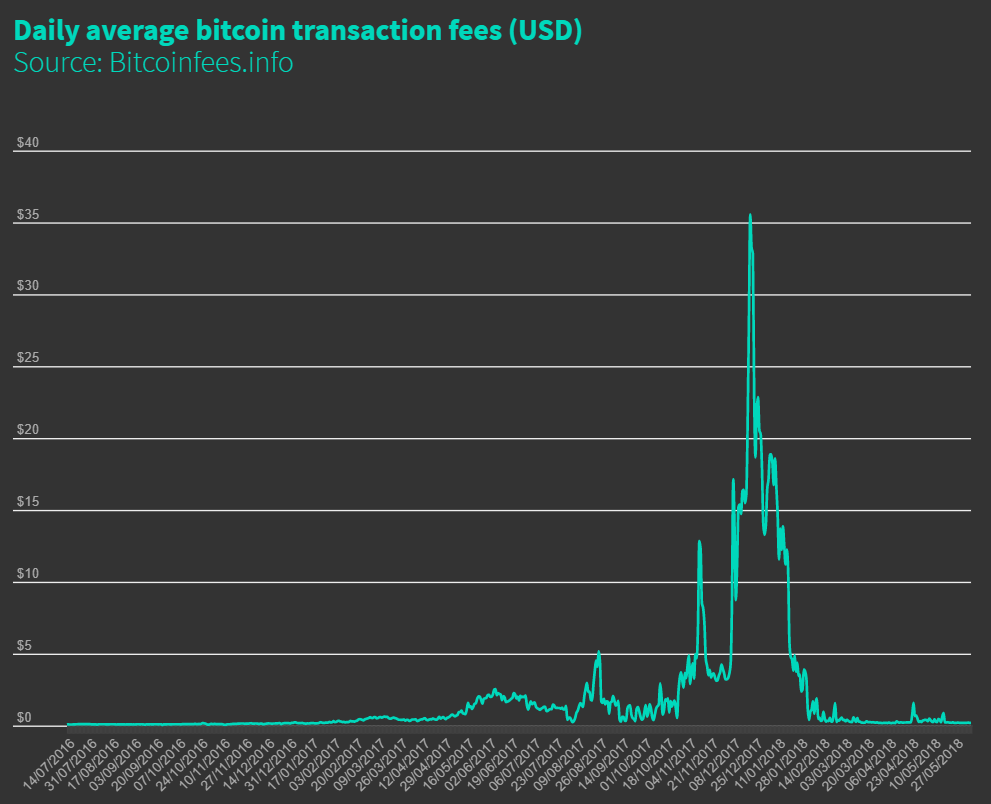
\includegraphics[width=7cm]{fee}
\caption{比特币日均每笔交易费用(美元)}
\end{figure}

\begin{figure}[htb]
\centering
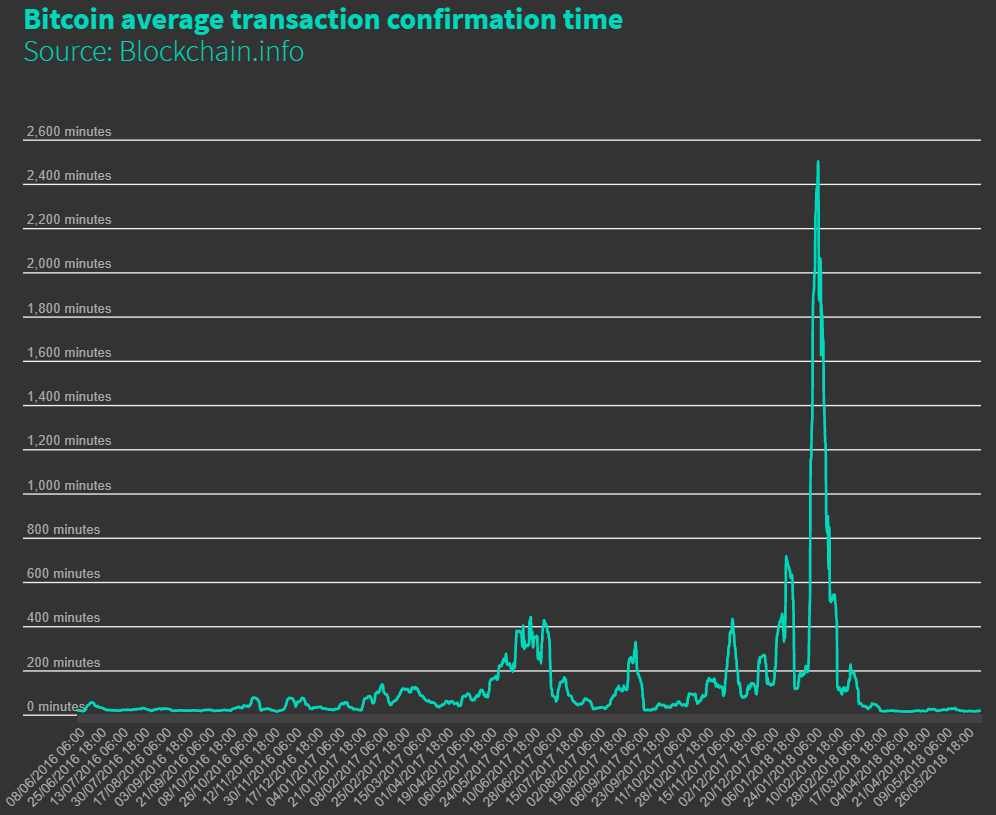
\includegraphics[width=7cm]{time}
\caption{比特币日均每笔交易确认时间(分钟)}
\end{figure}

\clearpage

\section{闪电网络}
\subsection{定义与特性}
闪电网络 \cite{poon2016bitcoin} 是一种轻量级的软件解决方案,用于扩展公共区块链与加密货币的互操作性。它是一个去中心化的系统,使得即时、大量的小额支付成为可能,且消除了将资金委托给受信任的第三方的风险。闪电网络最初由MIT媒体实验室针对比特币进行研发,但可以拓展应用于所有类似于比特币的区块链。具体来说,闪电网络的功能特性有如下四点。

\begin{enumerate}
	\item 即时支付。比特币将交易聚合成块,每10分钟进行一次。人们普遍认为,比特币在6次区块(耗时约1小时)确认后将被认为是安全的。显然这种确认时间不适合许多场景下的即时交易。而在闪电网络中,支付不需要经由区块确认,可以达到即时性和原子性。因此,闪电网络可以被广泛应用于销售终端、用户设备间交易以及其他需要即时支付的场景。

	\item 小额支付。闪电网络可以使得单笔交易额降至0.00000001比特币(低于0.01美分),且无需承担托管风险,而比特币的链上交易单笔最少数额要比这一值高数百倍。由于比特币单笔交易收费固定(远高于0.01美分),所以在链上进行小额交易是不切实际的。通过闪电网络,小额支付便可以进行,新的市场也得以开辟。


	\item 可扩展性。闪电网络将许多微支付通道连接成为网络,利用这个网络,比特币区块链在一台现代个人电脑上就可每天处理数十亿笔交易。大量的资金可以通过去中心化的方式在给定的交易通道内进行转移,这些通道并非在比特币之上建立独立的信任网络,每一笔经由通道的交易都是真实的比特币交易。

	\item 跨链交易。通过闪电网络,跨链间的原子性交易可以在链下实时发生,只要异构的区块链满足一致性准则。也即只要各个区块链支持相同的哈希函数,就有可能不在受信任的第三方托管下进行跨链交易。
\end{enumerate}

\subsection{关键技术}
闪电网络依赖于区块链的底层技术,通过使用原生的智能契约脚本,并进行真实的比特币交易,就可以创建一个安全的参与者网络,并以高容量和高速度进行交易。下面介绍闪电网络的两个核心概念:RSMC和HTLC。

\textbf{RSMC} (Recoverable Sequence Maturity Contract),即“可撤销的顺序成熟度合同”。首先假定交易双方之间存在一个微支付通道(资金池)。交易双方先预存一部分资金到微支付通道里,初始情况下双方的分配方案等于预存的金额。每次发生交易,需要对交易后产生资金分配结果共同进行确认,同时签字把旧版本的分配方案作废掉。任何一方需要提现时,可以将他手里双方签署过的交易结果写到区块链网络中,从而被确认。从这个过程中可以可以看到,只有在提现时候才需要通过区块链。

任何一个版本的方案都需要经过双方的签名认证才合法。任何一方在任何时候都可以提出提现,提现时需要提供一个双方都签名过的资金分配方案(意味着肯定是某次交易后的结果,被双方确认过,但未必是最新的结果)。在一定时间内,如果另外一方拿出证明表明这个方案其实之前被作废了(非最新的交易结果),则资金罚没给质疑方;否则按照提出方的结果进行分配。罚没机制可以确保了没人会故意拿一个旧的交易结果来提现。另外,即使双方都确认了某次提现,首先提出提现一方的资金到账时间要晚于对方,这就鼓励大家尽量都在链外完成交易。通过 RSMC,可以实现大量中间交易发生在链外。

下面举例说明RSMC的详细过程。假设Alice和Bob需要进行交易,那么在微支付通道建立时,双方必须有一定的资金沉淀在该通道上,我们假设目前通道中资金为:Alice: 0.4, Bob: 0.6,这样预存到通道的资金共有1.0 BTC,其中Alice拥有0.4 BTC,Bob拥有0.6 BTC。而支付通道的设立会记录在比特币的区块链上。某次,Bob决定向Alice支付0.1 BTC。在双方都签字认可的情况,链下支付通道的最新余额分配方案将变为{Alice:0.5, Bob:0.5},而且双方需要同时签字同意作废前一版本的余额分配方案{Alice:0.4, Bob:0.6},这样Alice就实际获得了0.5 BTC的控制权。

若Alice考虑到以后还会和Bob进行交易,那么她可以无需提取现在属于她的0.5 BTC,也无需在比特币区块链上更新已有变动的余额分配方案,因为若他们再次进行交易(如Alice向Bob支付0.2BTC)的话,他们仍然只需在链下对目的的余额分配方案达成一致,并设法作废前一版本的余额分配方案就行了。若Alice不打算再次和Bob进行交易并想动用通道的资金,她可以向区块链出示双方签字的余额分配方案。如果在规定时间内Bob未提出异议,区块链则会终止双方的支付通道并将资金按协议转入各自预先设立的提现地址。如果Bob在规定时间内提交证据证明Alice提交的是一个双方已同意作废的余额分配方案,那么Alice的资金将被罚没并给到Bob。

\textbf{HTLC} (Hashed Timelock Contract),即“哈希的带时钟的合约”,用于保证限时转账。通过智能合约,双方约定转账方先冻结一笔钱,并提供一个哈希值,如果在一定时间内有人能提出一个字符串,使得它哈希后的值跟已知值匹配(实际上意味着转账方授权了接收方来提现),则这笔钱转给接收方。

依然使用示例来说明该过程。如图所示,Alice(A)想给Darcy(D)发送0.05 BTC,但Alice和Darcy之间并没有微支付通道。但这没关系,闪电网络为Alice匹配了一条经过Bob(B)、Cady(C)到达Darcy的支付路径,该路径由Alice-Bob, Bob-Cady和Cady-Darcy这样三个微支付通道接力而成。Darcy生成一个哈希值$R$并将$Hash(R)$发送给Alice,Alice不需要知道$R$。$R$和$Hash(R)$的作用类似于钥匙和锁,只有匹配在一起才可开锁。Alice和Bob商定一个HTLC合约:只要Bob能在3天内向Alice出示正确的$R$,Alice会支付Bob 0.052 BTC;如果Bob做不到这点,这笔钱3天后自动退还Alice。同样地,Bob和Cady商定一个HTLC合约:只要Cady能在2天内向Bob出示哈希正确的$R$,Bob会支付Cady 0.051 BTC;如果Cady做不到这点,这笔钱到期自动退还Bob。最后,Cady和Darcy商定一个HTLC合约:只要Darcy能在1天内向Cady出示哈希正确的$R$,Cady会支付Darcy 0.05 BTC;如果Darcy做不到这点,这笔钱到期自动退还Cady。

方案确定好后,Darcy及时向Cady披露R并拿到0.05 BTC;现在Cady知道了$R$,她可以向Bob出示密码$R$并拿到0.051 BTC(差额部分的0.001 BTC成了Cady的佣金);Bob知道$R$后当然会向Alice出示并拿到他的那份 0.052 BTC,差额部分的 0.001 BTC成了Bob的佣金。大家可以看到,最终的结果是Alice通过闪电网络安全地向Darcy支付了 0.05 BTC,所付出的代价仅仅是支付给Bob和Cady(节点)的 0.002 BTC“过路费”(佣金)。

\begin{figure}[htb]
\centering
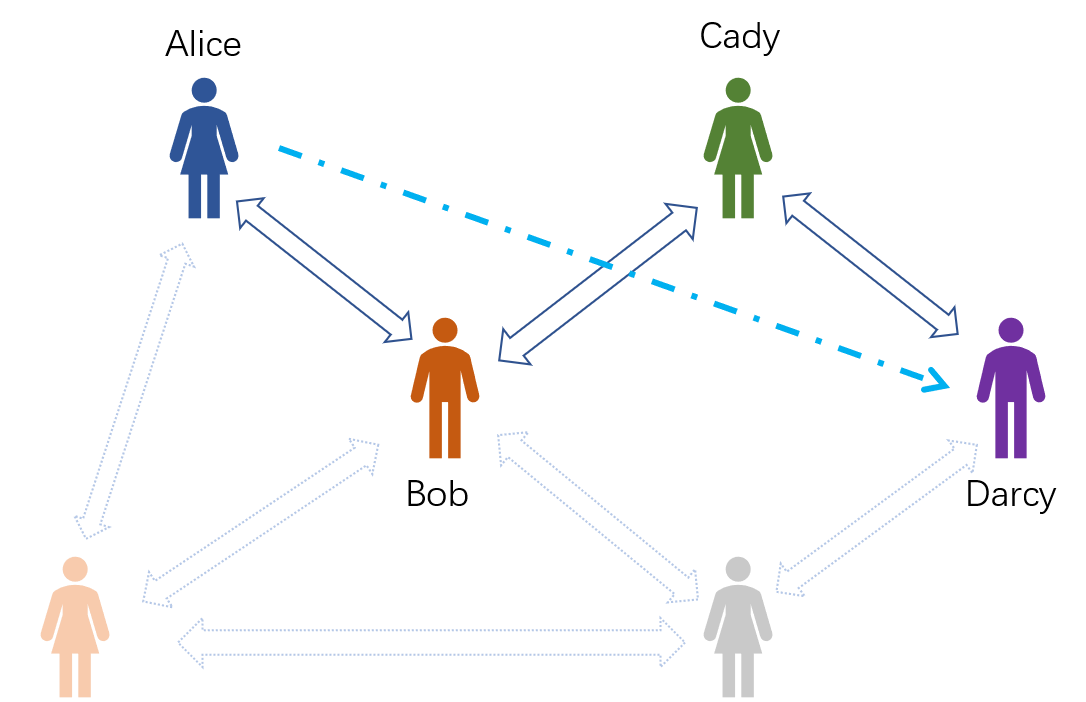
\includegraphics[width=9cm]{channels}
\caption{闪电网络微支付通道}
\end{figure}

\subsection{小结}
闪电网络的理念就是引入了一个类似于第三方中介且仅适用于高频次、小额交易的微支付通道。交易双方在这个微通道中必须先预存一定数量的保证金,而由区块链产生的智能合约(资金分配方案)进行监督评判。闪电网络中的所有交易动作都是发生在区块链之外,只有当需要提现时,才会将最终的交易结果写到区块链网络中并被最终确认。这大大降低了比特币区块链上的交易压力。

其中,RSMC 保障了两个人之间的直接交易可以在链下完成,HTLC 保障了任意两个人之间的转账都可以通过一条“支付”通道来完成。闪电网络整合这两种机制,就可以实现任意两个人之间的交易都在链下完成了。智能合约起到了中介的重要角色,而区块链网络则确保最终的交易结果被确认。

\section{路由协议}
\subsection{闪电网络中的通道寻优}
如第三部分所述,当交易双方之间没有直连的微支付通道时,需要将若干个支付通道连接,方可进行交易。在这个过程中,如何在发送方和接收方之间寻找到最优(或可接受)的路由通道将是一个挑战。在这个特定网络里,路由协议需要考虑路由费用、汇率以及可靠性等指标,使之可被接受。闪电网络使用主动式的路由协议,每个节点通过网络广播其邻居的信息(例如,广播通过网络连接的节点信息)。
\subsection{路由协议的种类}


1. 路由相关定义

2. PSTN,MANET,
由于PCN研究较少,故参考MANET(有一些相似之处)

3. 路由协议主要有5种,reactive, proactive, hybrid (i.e. a combination out of both: reactive and proactive), hierarchical and coordinate-based。

4. Flare,hybrid network. 列举我们的目标与Flare的区别。

\section{需求与算法选择}
为了找到合适的算法,对网络提出了几点需求:
1. Autonomy and self-reliance

2. Cost guaranties: Each

3. Time-lock guaranties

4. Flexibility

5. Prevent network partitioning

6. Real-time

7. Up-to-dateness

8. Lightweight and scalable

9. Trustlessness

10. Trustlessness

基于以上,我们选择/设计了AODV-based algorithm.

\clearpage

\bibliographystyle{IEEEtran}
\bibliography{ref}

\end{document}